\documentclass{standalone}
\usepackage{amssymb}
\usepackage{tikz}


\begin{document}
\begin{tikzpicture}
\node[inner sep=1cm] at (0, 0) {
\begin{tikzpicture}
	\node[inner sep=0] (tpc) at (0, 0) {
		\begin{tikzpicture}
			\node[inner sep=0] (figure) at (0, 0) {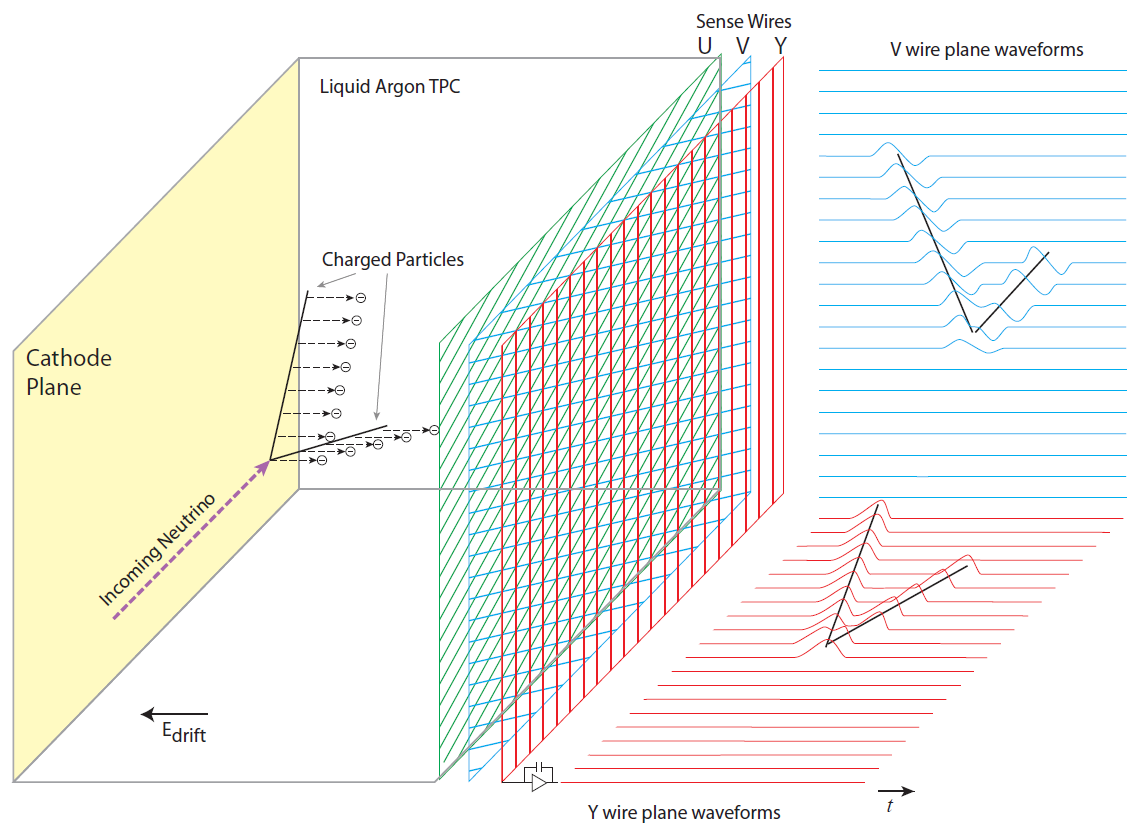
\includegraphics[trim=0 25 0 0, clip, width=13.5cm]{LArTPC.png}};
			\node[inner sep=0, anchor=south west] (label) at (figure.north west) {Liquid Argon Time-Projection Chamber (LArTPC)};
		\end{tikzpicture}
	};
	\node[inner sep=0, anchor=north west] (resp) at ([xshift=1cm]tpc.north east) {
		\begin{tikzpicture}
			\node[inner sep=0] (figure) at (0, 0){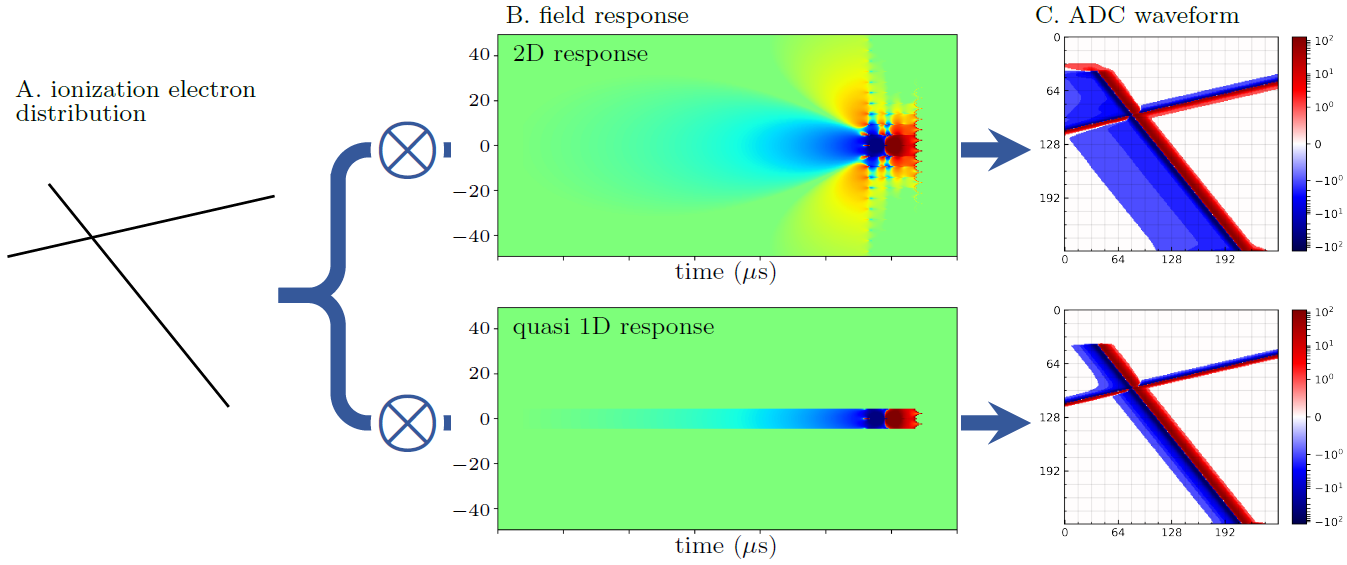
\includegraphics[width=13.5cm]{twoResponses.png}};
			\node[inner sep=0, anchor=south west] (label) at (figure.north west) {Two different (simulated) detector responses};
		\end{tikzpicture}
	};	
	\node[inner sep=0, anchor=north west] (eval) at ([yshift=-.5cm]tpc.south west) {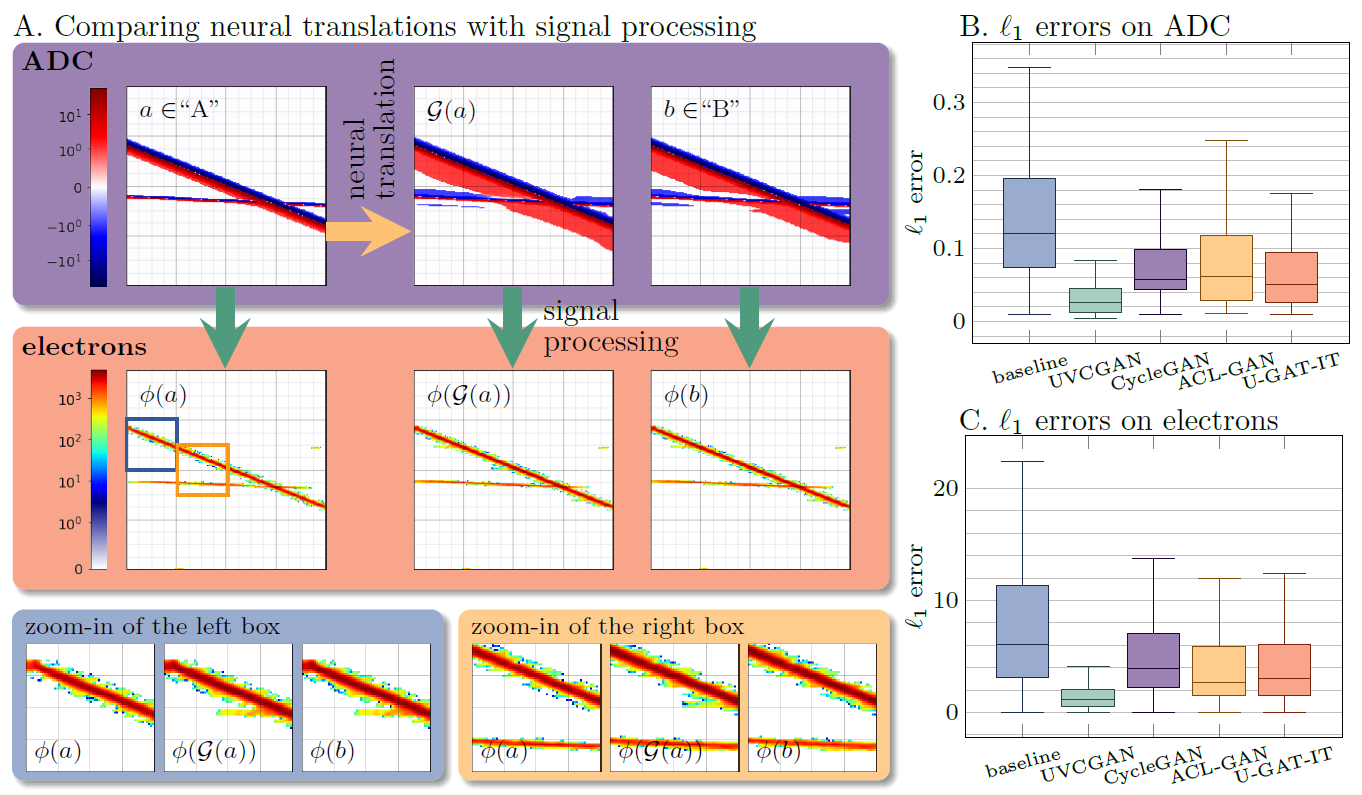
\includegraphics[width=13.5cm]{eval.png}};
	\node[inner sep=0, anchor=north west] (tran) at ([yshift=-.5cm]resp.south west){
		\begin{tikzpicture}
			\node[inner sep=0] (figure) at (0, 0) {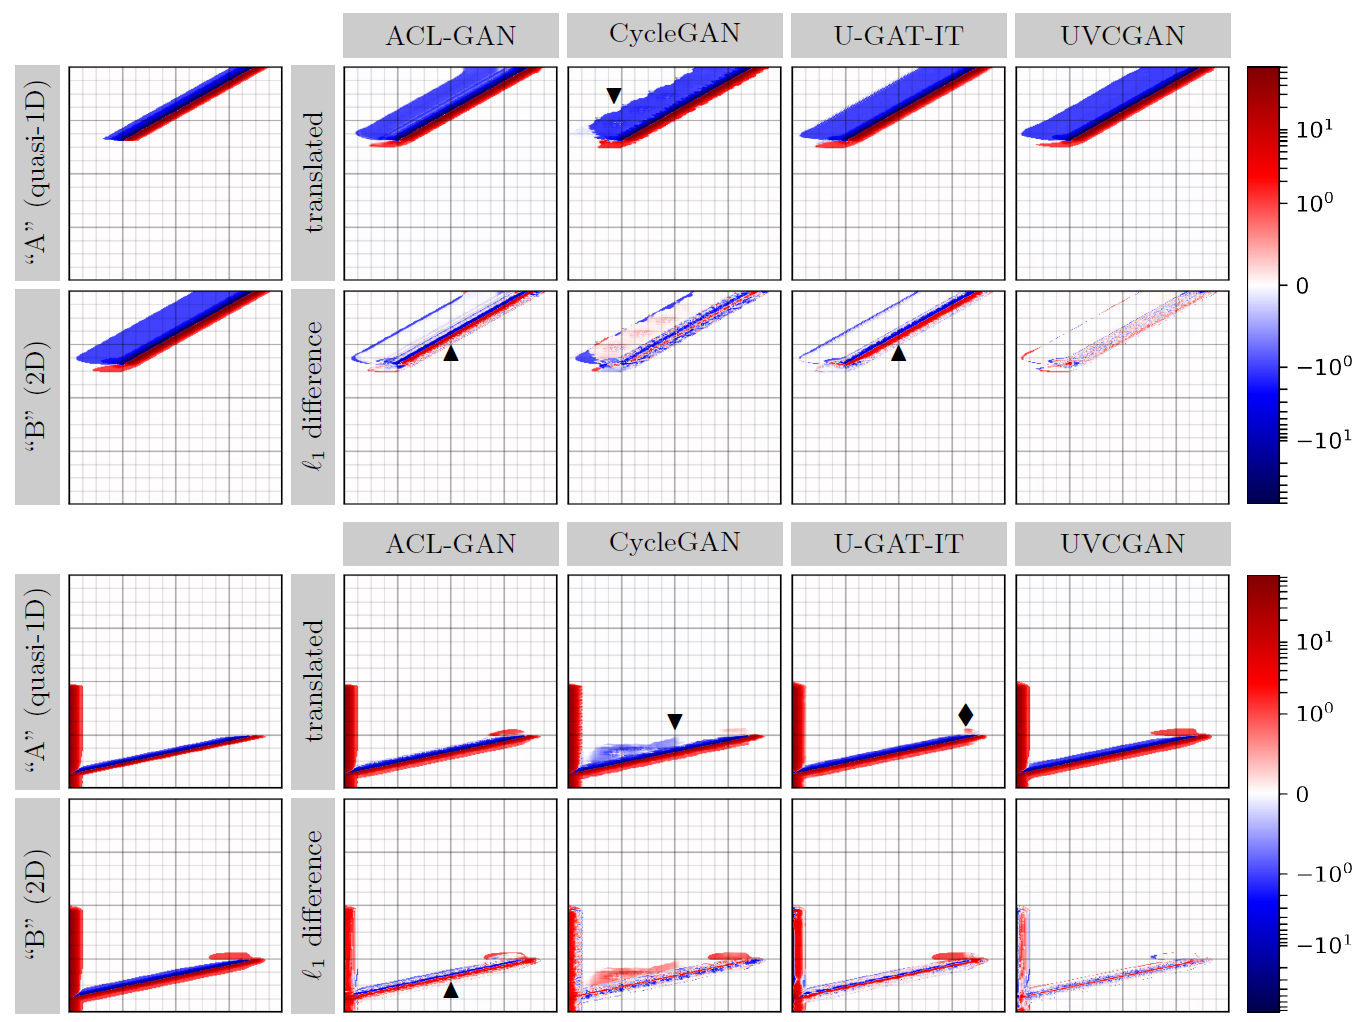
\includegraphics[width=13.5cm]{Translation_ADC.png}};
			\node[inner sep=0, anchor=south west, text width=13cm, align=left] (label) at (figure.north west) {Compare Translation Quality. 
        Defects appearing in the translations produced by the benchmarking algorithms are marked as:
        $\blacktriangledown$ for rugged track edge; 
        $\blacktriangle$ for big error in the core of the track where the signal is the strongest; 
        and $\blacklozenge$ for missing blob-shaped track tip.};
		\end{tikzpicture}
	};
\end{tikzpicture}
};
\end{tikzpicture}
\end{document}